\chapter{Руководство пользователя для системы}

\section*{Введение}

Система предназначена для автоматизированного отслеживания и представления
статусов кабинетов НИЯУ МИФИ. Это руководство поможет вам ознакомиться с
функциональностью телеграмм-бота системы.

\section*{Начало работы}

\subsection*{Доступ к боту}
Для начала работы откройте Telegram и найдите бота по названию
\texttt{@}mephi\_checker\_bot. Нажмите на ``Старт'' для инициализации бота.

\begin{figure}[h]
    \centering
    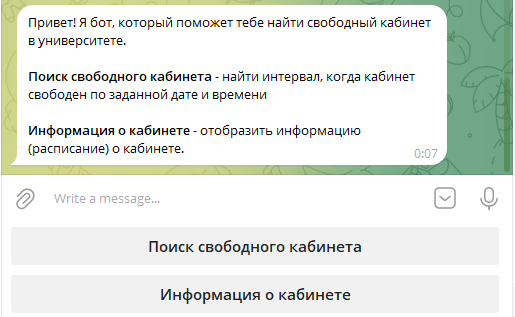
\includegraphics[scale=0.8]{img/1}
    \caption{}
    \label{fig:cp}
\end{figure}

\section*{Основные функции}
\begin{enumerate}
    \item Поиск свободных аудиторий
    \item Информация о конкретной аудитории
\end{enumerate}

\section*{Поиск свободных аудиторий}
Сначала необходимо выбрать корпус, в котором будет происходить поиск:
\begin{figure}[h]
    \centering
    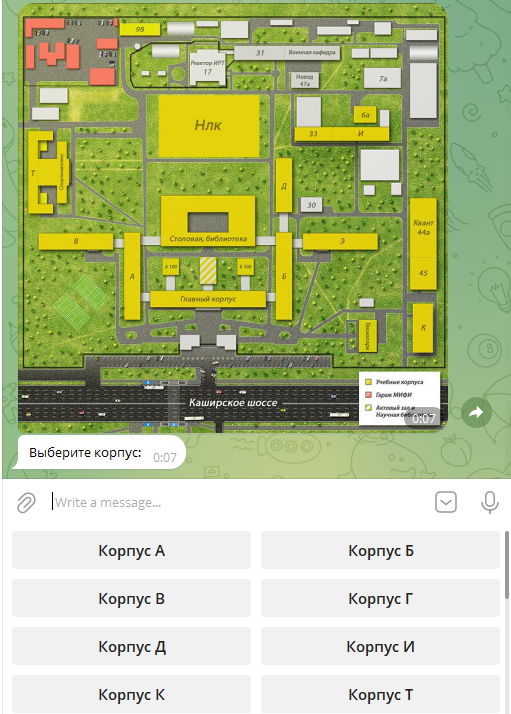
\includegraphics[scale=0.8]{img/2}
    \caption{Интерфейс бота(карта кабинета)}
    \label{fig:cp}
\end{figure}

После этого необходимо ввести дату поиска:
\begin{figure}[h]
    \centering
    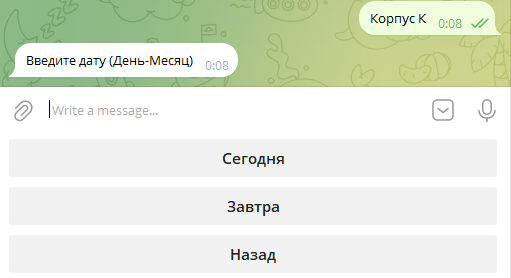
\includegraphics[scale=0.8]{img/3}
    \caption{Интерфейс бота(ввод даты)}
    \label{fig:cp}
\end{figure}

Последним этапом является ввод времени поиска:
\begin{figure}[h]
    \centering
    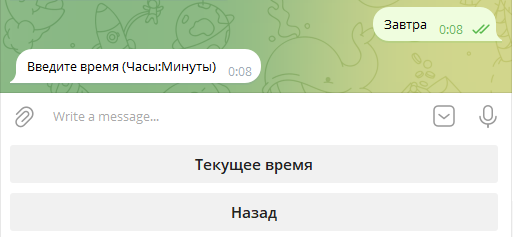
\includegraphics[scale=0.8]{img/4}
    \caption{Интерфейс бота(ввод времени)}
    \label{fig:cp}
\end{figure}

В результате пользователь получит список свободных кабинетов с
интервалом времени, когда он может его занять:
\begin{figure}[h]
    \centering
    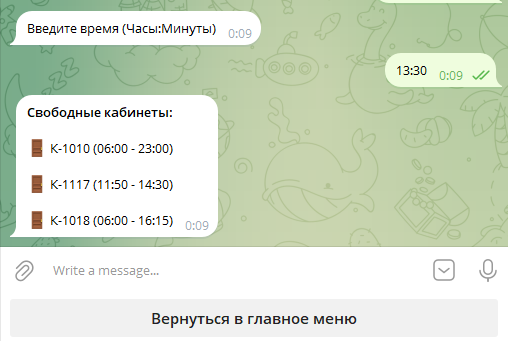
\includegraphics[scale=0.8]{img/5}
    \caption{Интерфейс бота(результат поиска)}
    \label{fig:cp}
\end{figure}

\section*{Информация о конкретной аудитории}
Сначала необходимо выбрать корпус, в котором будет происходить поиск:
\begin{figure}[h]
    \centering
    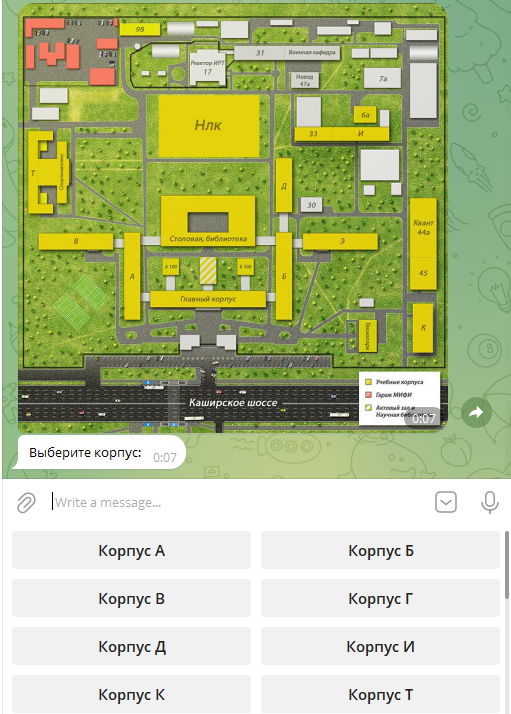
\includegraphics[scale=0.8]{img/2}
    \caption{Интерфейс бота(карта кабинета)}
    \label{fig:cp}
\end{figure}

После этого необходимо номер кабинета:
\begin{figure}[h]
    \centering
    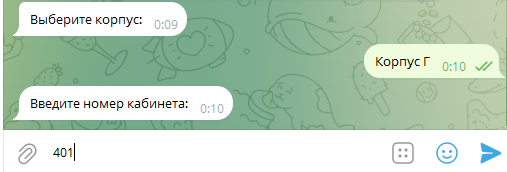
\includegraphics[scale=0.8]{img/6}
    \caption{Интерфейс бота(ввод номера кабинета)}
    \label{fig:cp}
\end{figure}


В результате пользователь получит полную информацию о кабинете:
\begin{figure}[h]
    \centering
    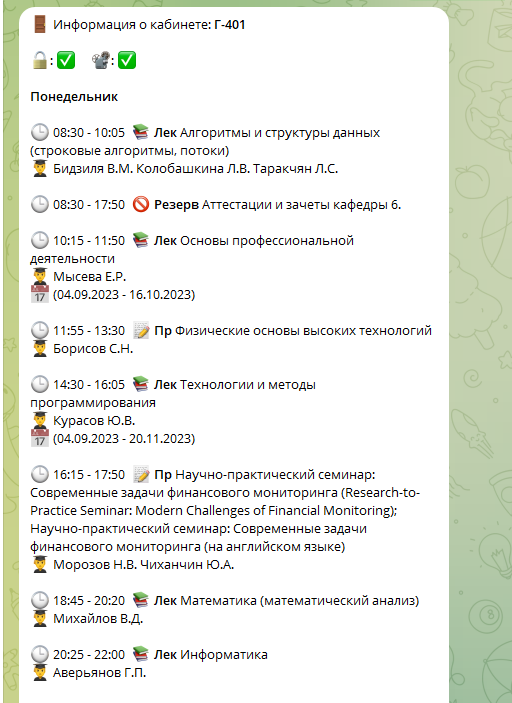
\includegraphics[scale=0.8]{img/7}
    \caption{Интерфейс бота(результат)}
    \label{fig:cp}
\end{figure}
